
% \chapter{Um apêndice}

    % Segundo a norma da ABNT (Associação Brasileira de Normas Técnicas), a definição e utilização de apêndices e anexos seguem critérios específicos para a organização de documentos acadêmicos e técnicos.
    
    % Apêndice: O apêndice é um texto ou documento elaborado pelo autor do trabalho com o objetivo de complementar sua argumentação, sem que seja essencial para a compreensão do conteúdo principal do documento. O uso de apêndices é indicado para incluir dados detalhados como questionários, modelos de formulários utilizados na pesquisa, descrições extensas de métodos ou técnicas, entre outros. Os apêndices são identificados por letras maiúsculas consecutivas, travessão e pelos respectivos títulos. A inclusão de apêndices visa a fornecer informações adicionais que possam ajudar na compreensão do estudo, mas cuja presença no texto principal poderia distrair ou desviar a atenção do leitor dos argumentos principais.

\chapter{Experiment 2}
    

    \section{Code for LLM-as-a-Judge}

\begin{lstlisting}[style=mystyle, language=Python, caption={C\'{o}digo para LLM-as-a-Judge}, label={code:llm-judge}]
class Confusion_Matrix(TypedDict):  # type: ignore
    true_positive: list[str]
    false_positive: list[str]
    true_negative: list[str]
    false_negative: list[str]

def calculate_metrics(llm, question, history):
    if type(question['Ground Truth']) == str:
        prompt_confusion_matrix = f"""                
            Voce recebera os seguintes parametros:
            Pergunta: a pergunta do usuario
            Resposta Ideal: a resposta considerada correta por um humano
            Resposta do sistema: a resposta fornecida pelo sistema baseado em IA

            Pegue a resposta do sistema, separe em afirmacoes e classifique cada afirmacao entre as opcoes abaixo:
            True Positive (TP): as afirmacoes corretas feitas pelo sistema, ou seja, que estao presentes na resposta ideal.
            False Positive (FP): as afirmacoes incorretas ou irrelevantes feitas pelo sistema, ou seja, que nao estao presentes na resposta ideal.

            Pegue a resposta ideal, separe em afirmacoes e classifique cada afirmacao entre as opcoes abaixo:
            True Negative (TN): Nao se aplica, deixar vazio.
            False Negative (FN): as afirmacoes que constam na resposta ideal, mas nao foram feitas pelo sistema.

            Importante:
            - Voce deve gerar listas de afirmacoes para cada categoria. 
            - Voce deve quebrar as respostas do sistema e a ideal em afirmacoes objetivas.
            - Se as respostas do sistema ou a ideal contiverem frases grandes com mtas afirmacoes, analisar cada afirmacao separadamente.
            - Uma afirmacao nao pode estar em mais de uma categoria.
            - Ignore coisas na resposta do sistema que nao sao afirmacoes objetivas, como por exemplo citacoes de fontes e links.

            Vamos la!

            ##################

            Pergunta: {{{{
            {question['Question']}
            }}}}

            Resposta ideal: {{{{
            {question['Ground Truth']}
            }}}}

            Resposta do sistema: {{{{
            {history[-1].content}
            }}}}
        """
        response = llm.with_structured_output(Confusion_Matrix).invoke(prompt_confusion_matrix)

        true_positive_count = len(response.get('true_positive', []))
        false_positive_count = len(response.get('false_positive', []))
        true_negative_count = len(response.get('true_negative', []))
        false_negative_count = len(response.get('false_negative', []))

        try:
            precision = true_positive_count / (true_positive_count + false_positive_count)
        except ZeroDivisionError:
            precision = 0
        
        try:
            recall = true_positive_count / (true_positive_count + false_negative_count)
        except ZeroDivisionError:
            recall = 0

        try:
            f1_score = 2 * (precision * recall) / (precision + recall)
        except ZeroDivisionError:
            f1_score = 0
            
        print("\\n\\nPrecision: "+str(precision))
        print("Recall: "+str(recall))
        print("F1 Score: "+str(f1_score))

        print("\\nAnswer Size Ratio: "+str(question['Answer Size (% of GT)']))

        state.precision = precision
        state.recall = recall
        state.f1_score = f1_score
        state.ground_truth = question['Ground Truth']
        state.statements = response
\end{lstlisting}

    \section{Results}
    \label{sec:exp2_appendix}

        % \subsection{Precision}

            % \subsubsection{Average Precision by Configuration}            % \begin{figure}[H]
            %     \centering
            %     \includegraphics{images_exp2/precision/bar_avg_precision_by_configuration.png}
            %     \caption{Average precision by configuration.}
            %     \label{fig:bar_avg_precision_by_configuration}
            % \end{figure}

            % \subsubsection{Average Precision by Model}
            % \begin{figure}[H]
            %     \centering
            %     \includegraphics{images_exp2/precision/bar_avg_precision_by_model.png}
            %     \caption{Average precision by model.}
            %     \label{fig:bar_avg_precision_by_model}
            % \end{figure}

            \subsubsection{Best Precision by Model and Configuration}
            \begin{figure}[H]
                \centering
                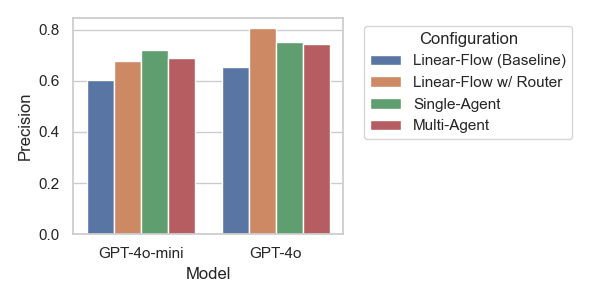
\includegraphics[scale=0.75]{images_exp2/precision/bar_best_precision_by_model_and_configuration.png}
                \caption{Best precision by model and configuration.}
                \label{fig:bar_best_precision_by_model_and_configuration}
            \end{figure}

            \subsubsection{Best Precision by Question Index and Configuration}
            \begin{figure}[H]
                \centering
                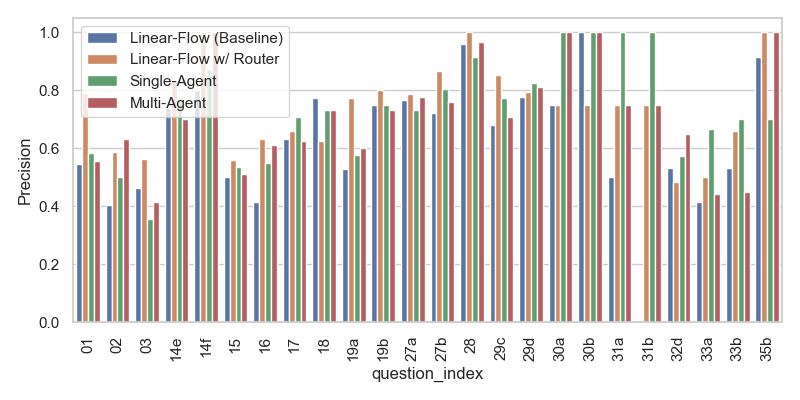
\includegraphics[scale=0.75]{images_exp2/precision/best_precision_by_question_index_and_configuration.png}
                \caption{Best precision by question index and configuration.}
                \label{fig:best_precision_by_question_index_and_configuration}
            \end{figure}

            \subsubsection{Best Precision by Question Index and Model}
            \begin{figure}[H]
                \centering
                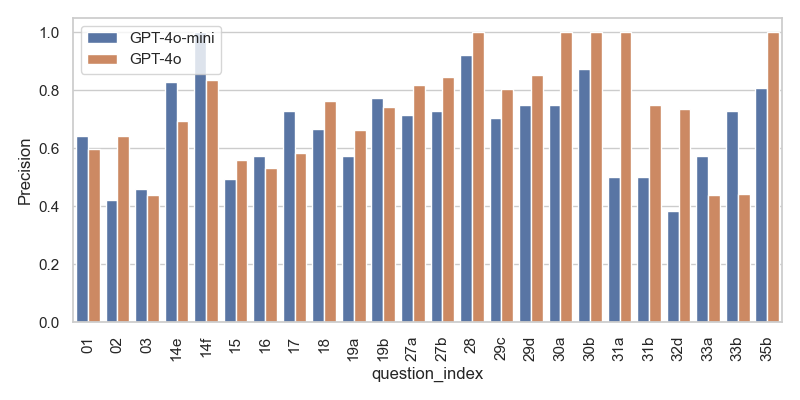
\includegraphics[scale=0.75]{images_exp2/precision/best_precision_by_question_index_and_model.png}
                \caption{Best precision by question index and model.}
                \label{fig:best_precision_by_question_index_and_model}
            \end{figure}

            \subsubsection{Facet Histogram of Precision by Model}
            \begin{figure}[H]
                \centering
                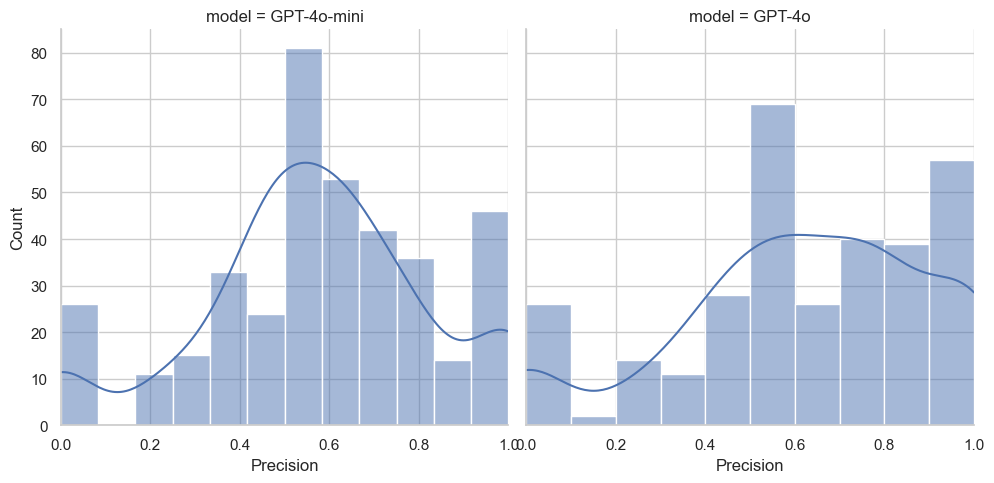
\includegraphics[width=\textwidth]{images_exp2/precision/facet_hist_precision_by_model.png}
                \caption{Facet histogram of precision by model.}
                \label{fig:facet_hist_precision_by_model}
            \end{figure}

            \subsubsection{Facet Histogram of Precision by Model (best of 3)}
            \begin{figure}[H]
                \centering
                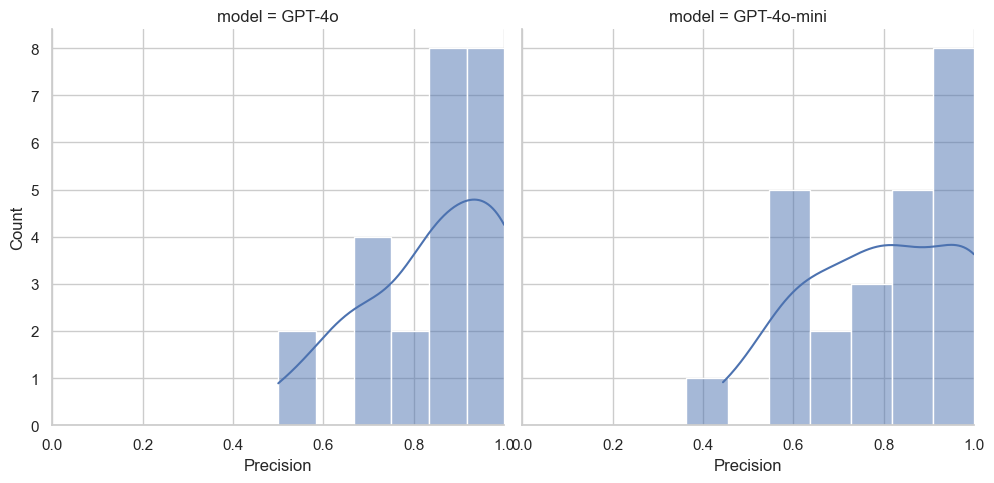
\includegraphics[width=\textwidth]{images_exp2/precision/facet_hist_precision_by_model_best_precision.png}
                \caption{Facet histogram of precision by model (best of 3).}
                \label{fig:facet_hist_precision_by_model_best_precision}
            \end{figure}

            % \subsubsection{Heatmap of Precision by Question and Model}
            % \begin{figure}[H]
            %     \centering
            %     \includegraphics[scale=0.75]{images_exp2/precision/heatmap_precision_by_question_and_model.png}
            %     \caption{Heatmap of precision by question and model.}
            %     \label{fig:heatmap_precision_by_question_and_model}
            % \end{figure}

            \subsubsection{Histogram of All Precisions}
            \begin{figure}[H]
                \centering
                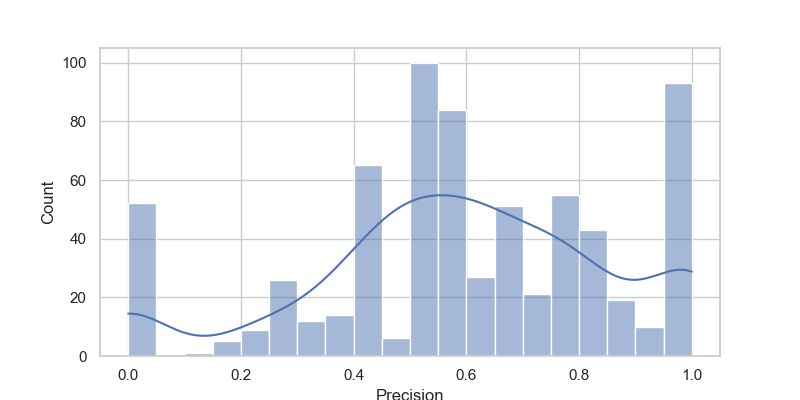
\includegraphics[scale=0.75]{images_exp2/precision/hist_precision_all.png}
                \caption{Histogram of all precisions.}
                \label{fig:hist_precision_all}
            \end{figure}

            \subsubsection{Line Plot of Precision by Question Index and Model}
            \begin{figure}[H]
                \centering
                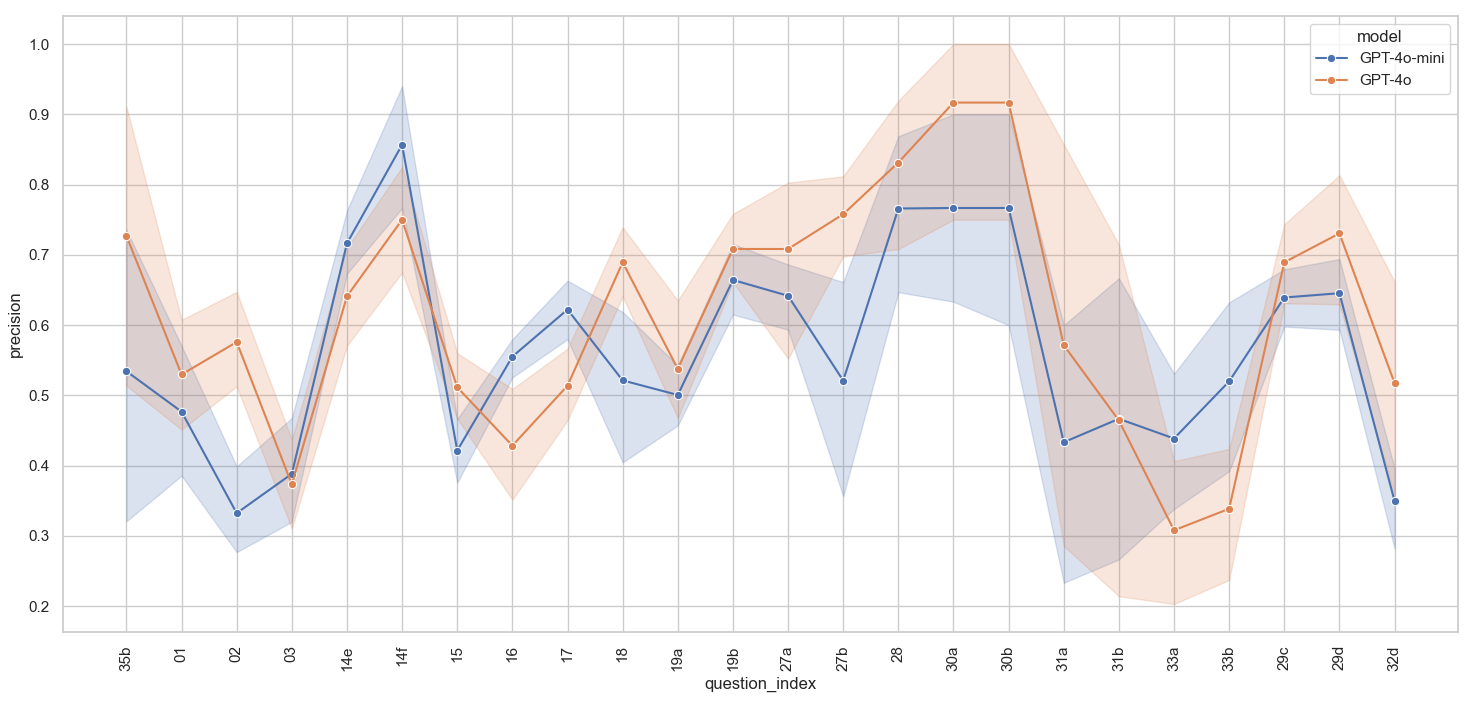
\includegraphics[width=\textwidth]{images_exp2/precision/line_precision_by_question_index_and_model.png}
                \caption{Line plot of precision by question index and model.}
                \label{fig:line_precision_by_question_index_and_model}
            \end{figure}

            \subsubsection{Boxplot of Precision by Model and Configuration}
            \begin{figure}[H]
                \centering
                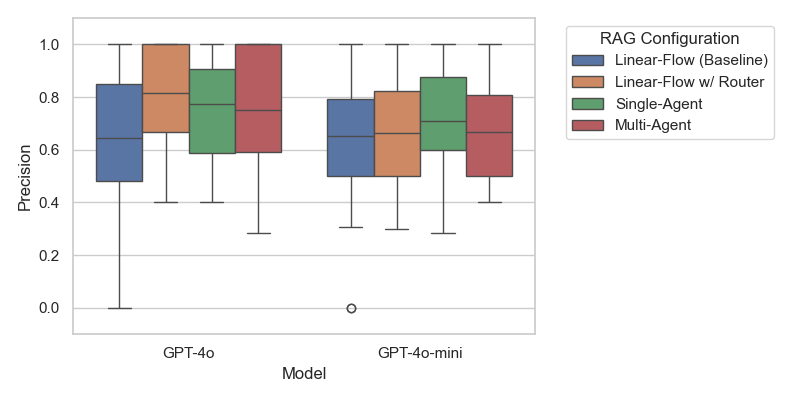
\includegraphics[scale=0.75]{images_exp2/precision/precision_boxplot_by_model_and_configuration.png}
                \caption{Boxplot of precision by model and configuration.}
                \label{fig:precision_boxplot_by_model_and_configuration}
            \end{figure}

            \subsubsection{Precision by Model}
            \begin{figure}[H]
                \centering
                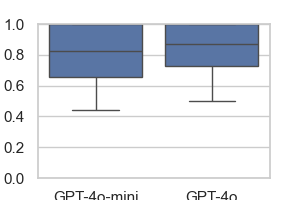
\includegraphics[scale=0.75]{images_exp2/precision/precision_by_model.png}
                \caption{Precision by model.}
                \label{fig:precision_by_model}
            \end{figure}

            \subsubsection{Precision by Model and Configuration}
            \begin{figure}[H]
                \centering
                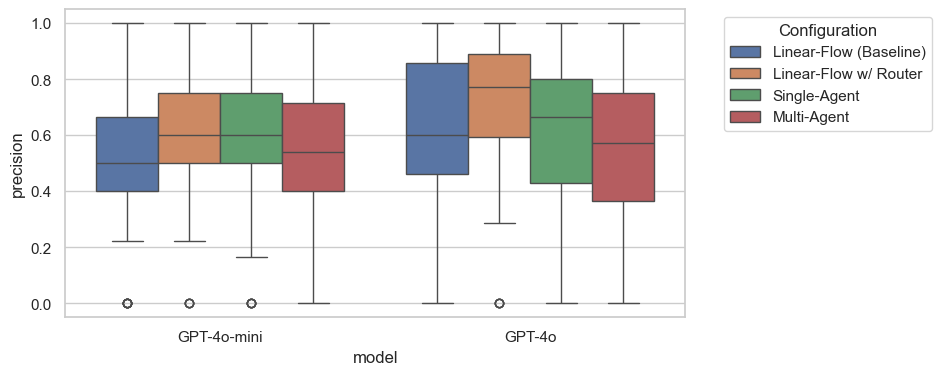
\includegraphics[scale=0.75]{images_exp2/precision/precision_by_model_and_configuration.png}
                \caption{Precision by model and configuration.}
                \label{fig:precision_by_model_and_configuration}
            \end{figure}

            \subsubsection{Line Plot of Precision by Question Index and Configuration}
            \begin{figure}[H]
                \centering
                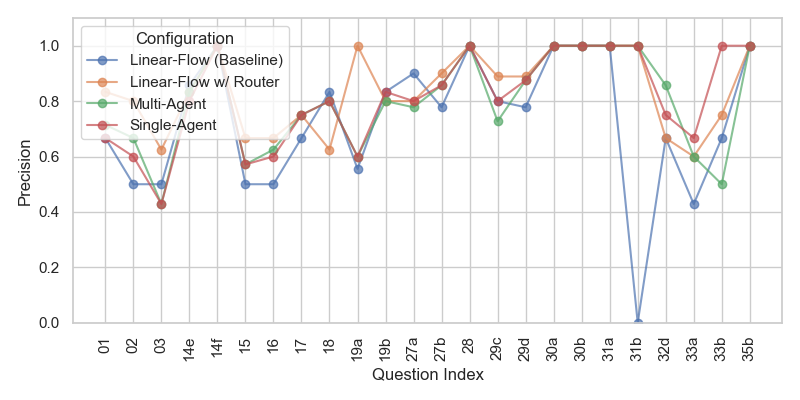
\includegraphics[width=\textwidth]{images_exp2/precision/precision_lineplot_by_question_index_and_configuration.png}
                \caption{Line plot of precision by question index and configuration.}
                \label{fig:precision_lineplot_by_question_index_and_configuration}
            \end{figure}

            \subsubsection{Scatter Plot of Precision vs. Total Time}
            \begin{figure}[H]
                \centering
                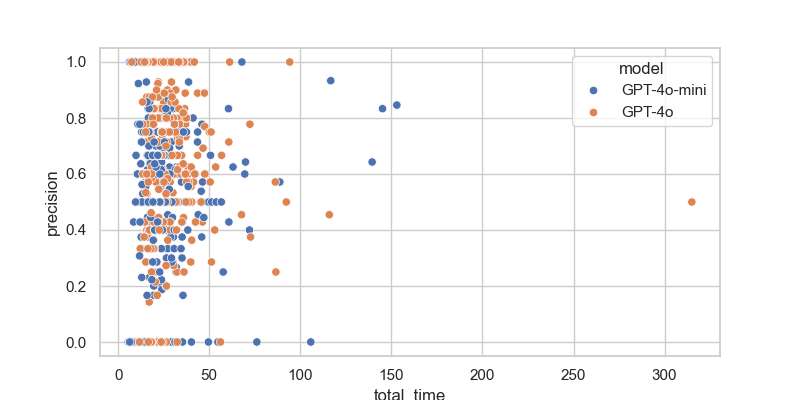
\includegraphics[scale=0.75]{images_exp2/precision/scatter_precision_vs_total_time.png}
                \caption{Scatter plot of precision vs. total time.}
                \label{fig:scatter_precision_vs_total_time}
            \end{figure}

            \subsubsection{Scatter Plot of Precision vs. Total Token Count Input}
            \begin{figure}[H]
                \centering
                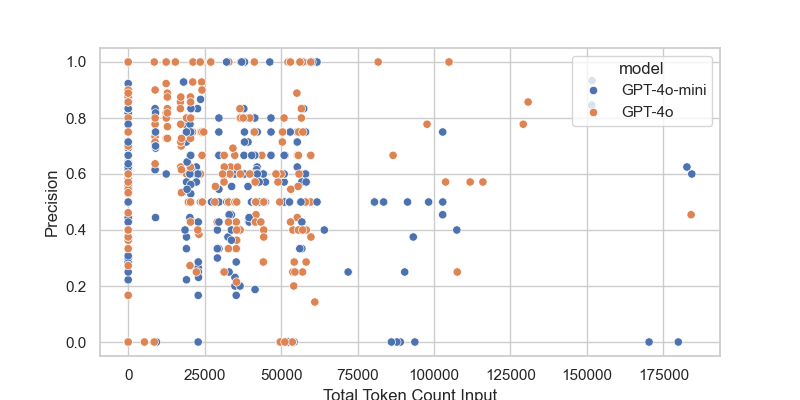
\includegraphics[scale=0.75]{images_exp2/precision/scatter_precision_vs_total_token_count_input.png}
                \caption{Scatter plot of precision vs. total token count input.}
                \label{fig:scatter_precision_vs_total_token_count_input}
            \end{figure}

            \subsubsection{Swarm Plot of Precision by Model and Configuration}
            \begin{figure}[H]
                \centering
                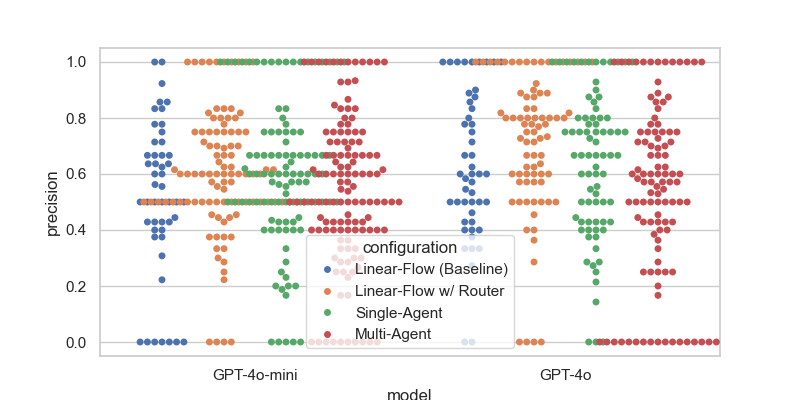
\includegraphics[scale=0.75]{images_exp2/precision/swarm_precision_by_model_and_configuration.png}
                \caption{Swarm plot of precision by model and configuration.}
                \label{fig:swarm_precision_by_model_and_configuration}
            \end{figure}

            \subsubsection{Violin Plot of Precision by Model and Configuration}
            \begin{figure}[H]
                \centering
                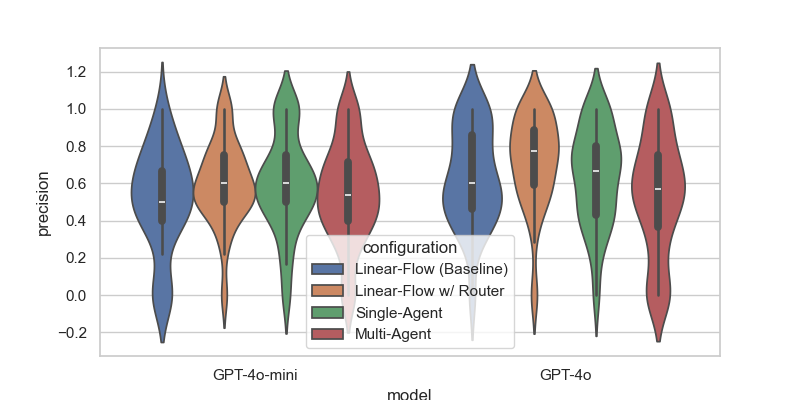
\includegraphics[scale=0.75]{images_exp2/precision/violin_precision_by_model_and_configuration.png}
                \caption{Violin plot of precision by model and configuration.}
                \label{fig:violin_precision_by_model_and_configuration}
            \end{figure}

        % \subsection{Recall}

        %     TEXT

        %     ...

        %     ... 

            
        %     TEXT

        %     ...

        %     ... 

        